\chapter{Implementierung}

\anno{max. 5 Seiten} %Ref hat 12

% Was lesen wir in diesem Kapitel?
% Warum muss ich das als Gutachter lesen
% Wie verknüpft sich der Inhalt mit dem vorhergehenden Kapitel?
% Welche Implmentierungsentscheidungen? Welche Alternativen? Vor- und Nachteile des eigenen Ansatzes?

% Highlight 1 der Implementierung
Wie bereits in Abschnitt \ref{sec:Probleme} angemerkt sind offene Implementationen von Web Application Firewalls eher die Ausnahme und selbst Umsetzungen der in Abschnitt \ref{sec:relatedwork} erwähnten Produkte sind praktisch nicht auffindbar. In diesem Kapitel gibt es einen kurzen Überblick wie die Vorschläge aus dem vorhergehenden Kapitel dennoch praktisch umgesetzt werden können.

Eine komplette Umsetzung ohne vorherige Basis wäre zeitlich (von einer einzelnen Person) nicht umsetzbar gewesen, daher sollte ein vorhandenes Open Source Produkt entsprechend erweitert werden. Bei der Auswahl wurden zuerst die zwei (leichtgewichtigen) Lösungen \emph{OWASP ESAPIFilter}\footnote{\url{https://owasp.org/www-project-enterprise-security-api/} abgerufen am 05.07.2023} und {SpringSecurity HttpFirewall}\footnote{\url{https://docs.spring.io/spring-security/reference/servlet/exploits/firewall.html} abgerufen am 05.07.2023} betrachtet. Beide Produkte verstehen sich als Ausgangsbasis für die Entwicklung sicherheitsrelevanter HTTP-(Servlet)-Filter auf Anwendungsebene, sämtliche Funktionalität muß jedoch vom Nutzer erst implementiert werden. Bei der Nutzung wäre ein erhöhter Arbeitsaufwand absehbar. Diogo Sampaio und Jorge Bernardino verglichen 2017 verfügbare WAFs die ebenfalls als Erweiterungskandidaten in Frage kamen (siehe Tabelle \ref{tab:my_vergos}).

% Tabelle ggf. in Anhang verschieben

\begin{table}[h]
  \centering
  \begin{tabular}{|c | c | c | c |} 
    \hline
    & \textbf{ModSecurity} & \textbf{WebCastellum} & \textbf{IronBee} \\ [0.5ex] 
    \hline
    Simple filtering & Yes & Yes & Yes \\ 
    \hline
    Regular expression based filtering & Yes &  & Yes \\
    \hline
    Auditing & Yes &  & Yes \\
    \hline
    Null byte attack prevention & Yes & Yes &  \\
    \hline
    URL Encryption & Yes & Yes &  \\ [1ex] 
    \hline
    Stateful Attack Detection & & Yes & Yes \\
    \hline
  \end{tabular}
  \caption{Vergleich Open Source Web Application Firewalls (aus \cite{Sampaio2017}) }
  \label{tab:my_vergos}
\end{table}

\emph{ModSecurity} und \emph{IronBee}s Stärken liegen in der regelbasierten Auswertung (\emph{regular expression based filtering}). Beide werden als Reverse-Proxy vor der eigentlichen Anwendung eingesetzt und sind keine HTTP-Servlet-Filter. Dies hat den Nachteil das kein Zugriff auf die eigentlichen Anwendungsdaten besteht und nur anhand des HTTP-Datenverkehrs gefiltert werden kann. \emph{WebCastellum} scheint hier Gutes aus beiden Welten bereit zustellen, zum einen (als Servlet-Filter) direkten Zugriff auf die Anwendungsdaten anzubieten, als auch regelbasiertes Filtern \emph{out-of-the-box}. \anno{Achtung! Sampaios Tabelle ist hier fehlerhaft! Übernehmen trotz Fehler?}
Mit Hinsicht auf einen späteren produktiven Einsatz wurde daher die Software \emph{WebCastellum} als Grundlage für die Implementierung der Firewall-Funktionalität gewählt.

\section{Vorarbeiten}

Leider haben WebCastellum und der CSIC2010 Datensatz eine Gemeinsamkeit - das Alter. Die derzeit aktuelle offizielle Version 1.8.3 von WebCastellum erschien bereits im Jahr 2009 und eine Weiterentwicklung fand seit dem nicht statt. Dennoch befindet sich das Produkt weiter in Verwendung und wird wohl auch in neuen Anwendungen genutzt, lässt zumindest die aktuelle Downloadstatistik (siehe \ref{fig:downloadwc}) vermuten. Insgesamt wurde das Binärpaket von WebCastellum in der Version 1.8.3 seit 2009 mehr als 8500 mal heruntergeladen (Stand vom 05. Juli 2023) - nicht berücksichtigt sind alle Vorgängerversionen und die Downloads über Repository-Dienste, wie z.B. Maven Central, stattfanden.

\begin{figure}[h]
  \centering
  \begin{gnuplot}[terminal=png,scale=.7]
    set datafile separator ','
    set xdata time
    set timefmt "%Y-%m"
    set xrange ["2009-01":"2023-09"]
    set format x "%b %y"
    set key autotitle columnhead
    plot '04_Implementierung/downloads.csv' using 1:2 with boxes fs solid 1.0 fc 'steelblue'
  \end{gnuplot}
  \caption{Download-Statistik SourceForge WebCastellum 1.8.3 binary}
  \label{fig:downloadwc}
\end{figure}

Vor den eigentlichen Arbeiten waren also noch ein paar kleinere Vorarbeiten notwendig. In einem ersten Schritt wurde der Quellcode aus dem SourceForge-Repository heruntergeladen und in ein eigenes git-Repository\footnote{\url{https://github.com/devtty/webcastellum/} abgerufen am 05.07.2023} übertragen. 

\subsection{Version 1.8.4. - Review des Quellcode und IT-Sicherheit}
Während die Binär-Distribution mit der Versionsnummer 1.8.3 verteilt wird, sind die Quellen bereits mit der nächsten Minor-Version versehen. Diese lassen sich auch fast problemlos kompilieren und zu einem verwendungsfähigen Paket zusammenbauen. Das Projekt hat nur sehr wenig Abhängigkeiten zu weiteren Bibliotheken und diese (laut durchgeführtem OWASP dependency-check) keine bekannten Schwachstellen. Etwas problematisch ist die Abhängigkeit zu älteren Bibliotheken (\emph{javax.jms} und \emph{javax.mail}), da diese nicht mehr (direkt) über den Standard-Build-Mechanismus verfügbar sind, sich aber über Umwege auftreiben lassen.

Im weiteren Verlauf des Projektes wurden die Quellen noch einer Codeanalyse auf der Sonarcloud-Plattform \footnote{\footnote{\url{https://sonarcloud.io/project/overview?id=devtty_webcastellum} abgerufen am 05.07.2023}} unterzogen. Insgesamt fielen dabei im Quelltext sechs direkte Schwachstellen und 58 potentielle Schwachstellen (siehe \ref{fig:my_sonar1}) auf. Bei den direkten Schwachstellen handelt es sich um:

\begin{itemize}
    \item 3 x Verwendung schwacher Kryptographie (hier AES; Cryptographic Failures / Security Misconfiguration )
    \item 2 x Ausgabe der Session-ID in Log-Dateien (Insecure Design/Broken Authentication)
    \item 1 x XML External Entity Injection Attack (Security Misconfiguration / XML External Entities (XXE))
\end{itemize}

Wobei die XXE-Attacke von Sonar als Blocker eingestuft wird. Bei den 58 Security Hotspots handelt es sich meistens um direkte Ausgaben im Fehlerfall (\verb=printStackTrace()=) mit der Bitte zur Überprüfung das diese im Produktivbetrieb nicht ausgegeben werden. 

Inklusive Code Smells bemängelt Sonar den Quellcode in insgesamt 2657 Fällen und berechnet die angehäuften technischen Schulden auf 52 Personen-Tage Nacharbeit. 

\begin{figure}
    \centering
    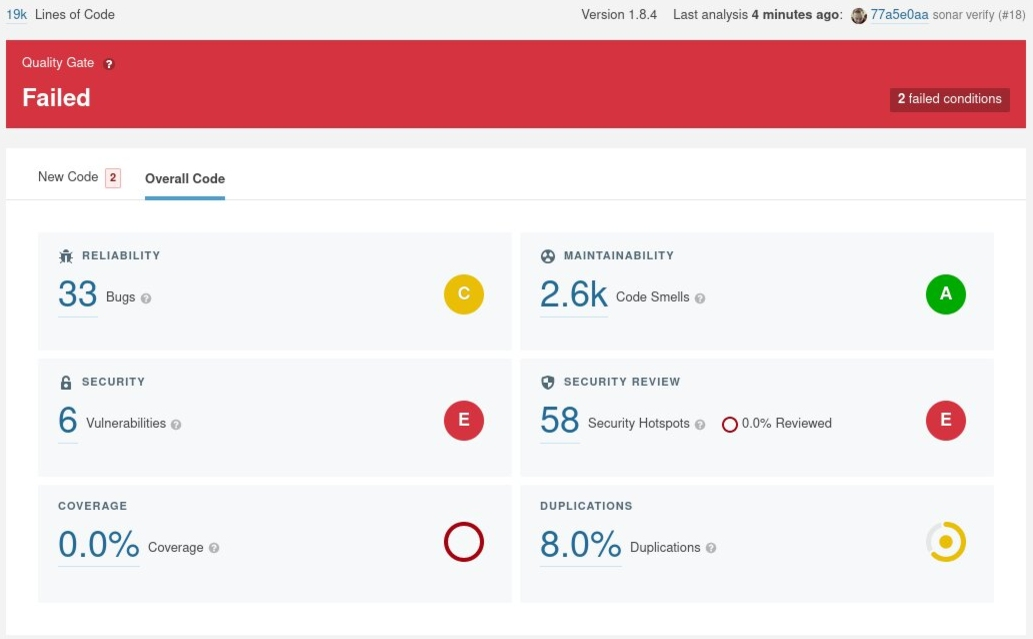
\includegraphics[width=\textwidth]{first_sonar2.jpg}
    \caption{SonarCloud erste Sichtung}
    \label{fig:my_sonar1}
\end{figure}

\begin{figure}
    \centering
    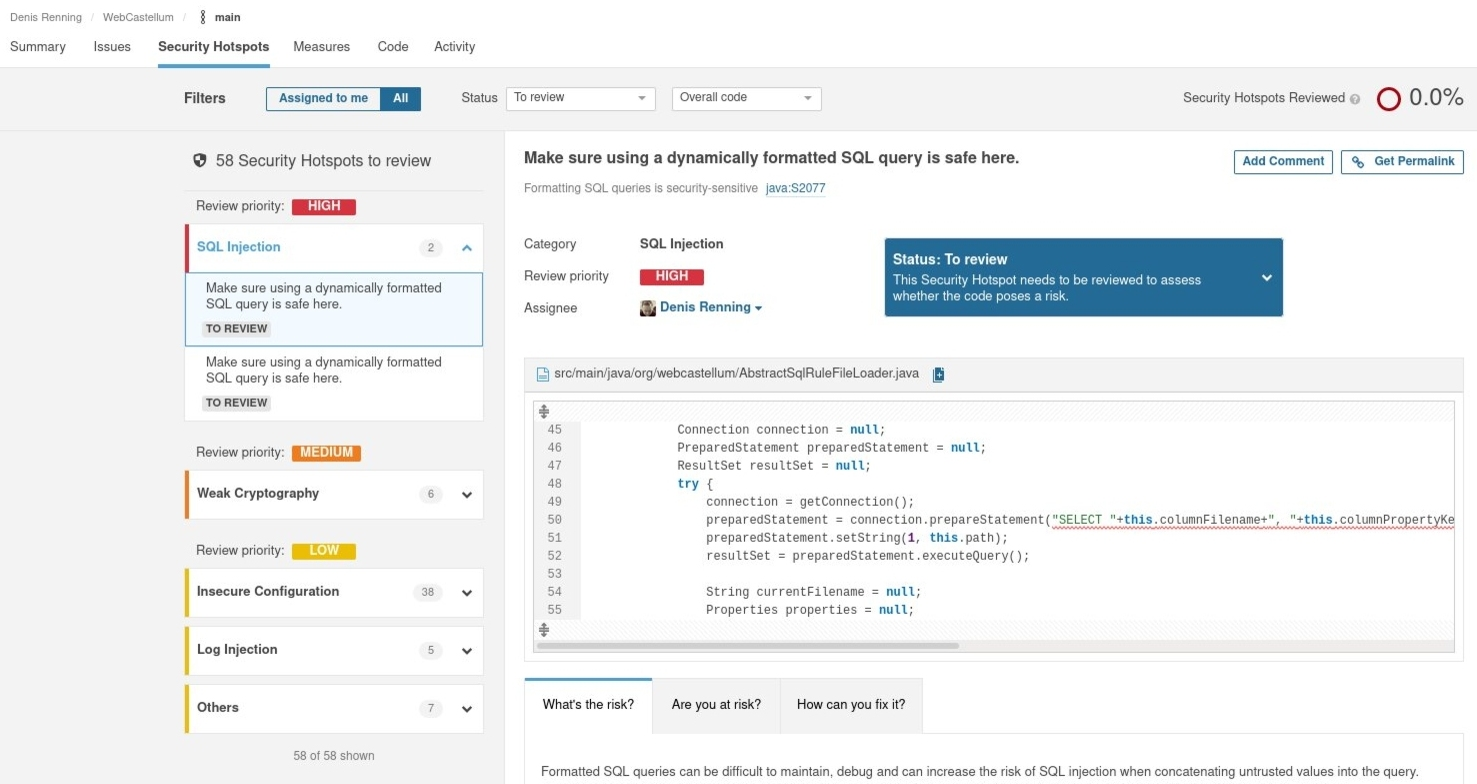
\includegraphics[width=\textwidth]{first_sonar_sql.jpg}
    \caption{SonarCloud SQL-Injection}
    \label{fig:my_sonar2}
\end{figure}



\subsection{Unit-Tests etc.}
\subsection{Fehlerbereinigung}

% Highlight 2 der Implementierung
\section{Zentralisierung}
\begin{figure}[ht]
    \centering
    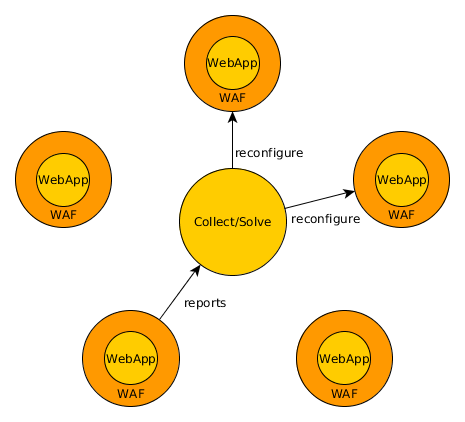
\includegraphics[width=8cm]{central.png}
    \caption{Arbeit der WAFs im Verbund}
    \label{fig:my_verbund}
\end{figure}

\begin{figure}[bht]
  \begin{center}
    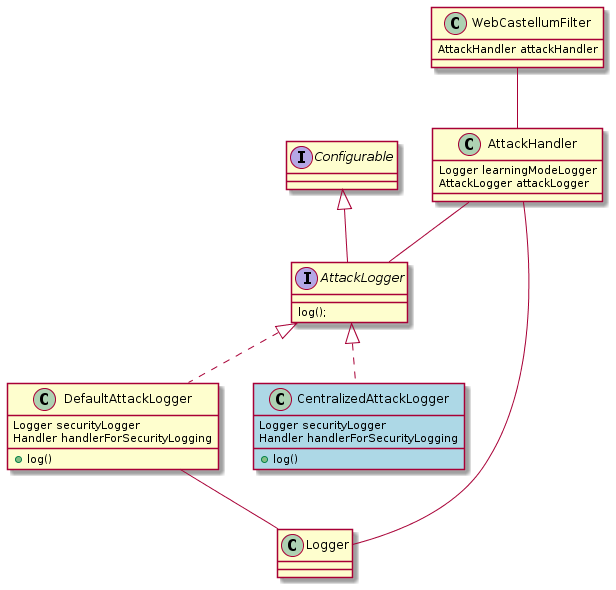
\includegraphics[width=12cm]{classp}
    \caption{Implementierung Nachrichtenversand}
    \label{fig.impversand}
  \end{center}
\end{figure}

\begin{figure}[h]
  \begin{center}
    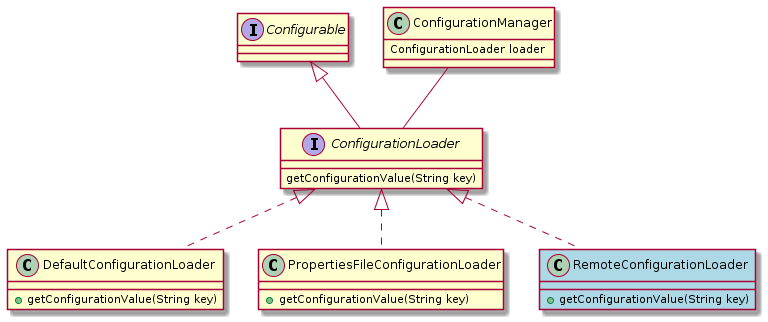
\includegraphics[width=14cm]{configclasses}
    \caption{Implementierung Konfiguration}
    \label{fig.impkonfig}
  \end{center}
\end{figure}



\section{ML-Fähigkeit}

\begin{figure}[h]
    \centering
    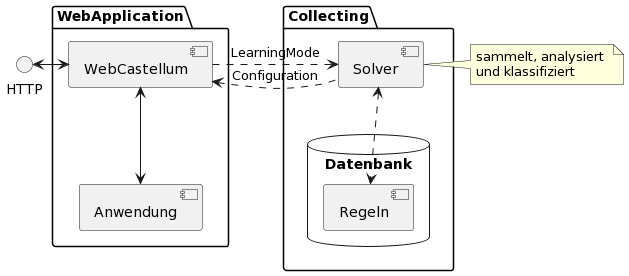
\includegraphics[width=9cm]{webcastellumcentral.png}
    \caption{Komponentendiagramm für zentrale Klassifizierung}
    \label{fig:my_future}
\end{figure}


% Highlight des Deployments beim Kunden

% Zusammenfassung: ca. 0,5 Seiten
\section{Zusammenfassung}

% Was haben wir in diesem Kapitel gelernt?
% Wie passt das zur Zielstellung der Arbeit?
% Wie passt das zum nächsten Kapitel?